\documentclass[11pt,fleqn,twoside]{article}

\newif\ifreport
\reporttrue

\usepackage[english,german]{babel}
\usepackage{derireport}

\usepackage{alltt}
\usepackage{verbatim}
\usepackage{graphicx}
\usepackage{url}
\usepackage{subfigure}
\usepackage{listings}
\usepackage{color}
\usepackage{lscape}
\usepackage{xspace}
\usepackage{latexsym}
\usepackage{rotating}
\usepackage{enumitem}


\definecolor{lightblue}{rgb}{.3,.5,1}
\definecolor{orange}{rgb}{1,.7,0}
\definecolor{darkorange}{rgb}{1,.4,0}
\definecolor{darkgreen}{rgb}{0,.4,0}
\definecolor{darkblue}{rgb}{0,0,.4}
\definecolor{darkred}{rgb}{.56,0,0}
\definecolor{gray}{rgb}{.2,.2,.2}
\definecolor{shadecolor}{gray}{0.7}

%% define RDFa look and feel
\lstdefinelanguage{RDFa}{
      morekeywords=[1]{about, ref, rel, content, property, href, resource, datatype, typeof},
      morestring=[b]",
      sensitive=false%
}[keywords,comments,strings]

\lstset{
      basicstyle = \scriptsize \ttfamily,%
      keywordstyle = [1]\color{darkgreen},%
      stringstyle  = \ttfamily\color{darkred},%
      commentstyle = \itshape\color{darkblue},%
      showstringspaces = false,%
%     fancyvrb = true,%
      firstnumber = auto, stepnumber=1, numbersep=5pt,%
      numbers=left, numberstyle=\tiny \ttfamily,
      frame = shadowbox, frameround = ffff, rulesepcolor = \color{shadecolor},
      breaklines=true, breakatwhitespace=true,%
%     prebreak=\textellipsis,postbreak=\textellipsis,%
      emphstyle = \color{red}\underbar, emphstyle = {[2]\color{blue}\underbar},%
      extendedchars = true, inputencoding = utf8,%
%     backgroundcolor=\color{shadecolor},
      xleftmargin=20pt, xrightmargin=10pt,
      captionpos = b
}


%% define N3 look and feel
\lstdefinelanguage{N3}{
      morekeywords=[1]{@prefix, a },
      morestring=[b]",
      morecomment=[s]{<}{>}, % missusing comments for URIrefs
      otherkeywords={^, [, ], (, )},%
      %otherkeywords=[2]{<, >},% for URIrefs
      sensitive=false%
}[keywords,comments,strings]

\lstset{
      basicstyle = \scriptsize \ttfamily,%
      keywordstyle = [1]\bfseries\color{darkgreen},%
      stringstyle  = \ttfamily\color{darkred},%
      commentstyle = \itshape\color{darkblue},%
      showstringspaces = false,%
%     fancyvrb = true,%
      firstnumber = auto, stepnumber=1, numbersep=5pt,%
      numbers=left, numberstyle=\tiny \ttfamily,
      frame = shadowbox, frameround = ffff, rulesepcolor = \color{shadecolor},
      breaklines=true, breakatwhitespace=true,%
%      prebreak=\textellipsis,postbreak=\textellipsis,%
      emphstyle = \color{red}\underbar, emphstyle = {[2]\color{blue}\underbar},%
      extendedchars = true, inputencoding = utf8,%
%     backgroundcolor=\color{shadecolor},
      xleftmargin=5pt, xrightmargin=2pt,
      captionpos = b
}



\foreignreport

% Body of the report is Foreign (English) or German ...
% Only relevant, of full report is not English
%\foreignbody

%%%%%%%%%%%%%%%%%%%%%%%%%%%%%%%%%%%%%%%%%
% Macros

 \newtheorem{theorem}{Theorem}[section]
 \newtheorem{proposition}[theorem]{Proposition}
 \newtheorem{corollary}[theorem]{Corollary}
 \newtheorem{lemma}[theorem]{Lemma}

 \newtheorem{example}{Example}[section]
 \newtheorem{definition}{Definition}[section]

%\newcommand{\qed}[0]{\hspace*{1em}\hbox{\proofbox}}

% \newtheorem{zdefinition}{Definition}[section]
% \newenvironment{definition}[1][\mbox{}]{\begin{zdefinition}\begin{rm}#1}{\end{rm}\end{zdefinition}}

% \newtheorem{zexample}{Example}[section]
% \newenvironment{example}[1][\mbox{}]{\begin{zexample}\begin{rm}#1}{\end{rm}\end{zexample}}


 %% No numbered paragraphs
 \setcounter{secnumdepth}{3}

%%%%%%%%%%%%%%%%%%%%%%%%%%%%%%%%%%%%%%%%%%%%%%%%%%%%%%%%%%%%%%%%%%%%%%%%%%%%%%%%%%



%
% This is the title of the report, shown on the cover:
%

\title{Developing in the Cloud}

% The names of the authors must be specified for the title page,
% where they appear without the affiliations.

\authornames{
Aftab Iqbal
\and
Michael Hausenblas
\and
Stefan Decker
}


\innertitle{Developing in the Cloud}

%  The authors appear with affiliations.
%  Thanks may be given for individual acknowledgements.
\author{
Aftab Iqbal\affiliation{
DERI, National University of Ireland, Galway, Ireland.
\mbox{firstname.lastname@deri.org}
}
\and
Michael Hausenblas\footnotemark[1]
\and
Stefan Decker\footnotemark[1]
}

% General acknowledgements, appearing only on the inside titlepage.
% Must be one continuous paragraph.
% If you want to make two or more paragraphs,
% use \\*[\parskip] for new line, but do not leave a line empty.
%

\acknowledgement{
This work has been carried out in the Linked Data Research Centre (LiDRC) and has been supported by Science Foundation Ireland under Lion 2 and the European Commission's FP7 Support Action LOD-Around-The-Clock (LATC), project no. 256975, Intelligent Information Management (ICT-2009.4.3).
}

%
% Abstract must also be one continuous paragraph.
% If you want to make two or more paragraphs,
% use \\*[\parskip] for new line and \hspace*{1.5em} for indentation,
% but do not leave a line empty.
%

\abstract{
%In this ever-changing world of software development, software developers are required to keep up with technologies, methodologies and trends. They use a variety of software tools and development frameworks in their day to day software development tasks. Managing and monitoring the development activities using different project management and collaborative tools allow developers to be geographically distributed.
%With the emergence of cloud computing, few efforts have emerged which started to offer cloud-based development infrastructure hence enabling editing, build and deployment of software applications using browser-based IDE in the cloud. This trend can significantly change the way software development is currently being carried out. In this report, we review the current state of the art of those browser-based IDEs and outline features, limitations and challenges which these browser-based IDEs have to deal with in the near future.
With cloud computing as an infrastructure model maturing, more and more efforts around cloud-based software development are emerging. In this model, a cloud-based environment enables developers to edit, test and deploy Web applications through a Web browser. We consider this tool stack to be disruptive in its nature, changing the way software development is being carried out and opening up new opportunities for service providers as well as (teams of) developers. In this report, we review the state of the art of cloud-based software development environments, analyse their shortcomings and provide a roadmap for the next generation of cloud-based development tools.
\\*[\parskip]
~
\\*[\parskip]
{\bf Keywords:} cloud computing, agile software development, collaborative software development, integrated development environment.
}

% \begin{comment}
% With the growing interest in the usage of online social networking sites: developers of FOSS projects, users and others interested quite often get in touch with each other using social platforms for example, by following the tweets on Twitter or by joining the project's Facebook group community to discuss, debate, share experiences or post questions related to a FOSS project along-with the traditional ways of communication i.e. discussion forums, mailing lists, IRC channels etc. In order to bridge the connections between FOSS projects and the social networking sites, we proposed a novel way of interlinking the heterogeneous data islands (i.e. social networking sites and the FOSS project repositories) using the Linked Data principles. By enabling interlinking among these heterogeneous data islands, we are able to understand the social and development activities of the developers related to a FOSS project based on the assumption that the developers of the FOSS projects are also using the social networking sites.
% \\*[\parskip]\hspace*{1.5em}
% FOSS projects are dynamic in nature: developers/contributors contribute to a project for a certain period of time and later left the project or join other project of high interest. So, FOSS projects always welcome contributors who can contribute to the project by submitting source-code patches, fixing particular bugs or even reporting bugs. Given the dynamic nature of FOSS projects, we investigates if such a generic FOSS model can be applied to bespoke systems, where a team of developers can be built dynamically from a list of potential and interested developers having expertise in certain technologies required to develop the bespoke system.
% %FOSS developers/contributors very often work on multiple projects which they find personally interested [ref required!].
% \\*[\parskip]\hspace*{1.5em}
% To evaluate our proposed approach, we harnessed data from social networking sites and software repositories and interlinked them where necessary. Further, we exploited our interlinked datasets to build the developer's expert profile which was later used to recommend potential developers for a project seeking developers/contributors.
% \\*[\parskip]
% ~
% \\*[\parskip]
% \end{comment}

\deritr{2012-10-06}
% Give different versions separated by semicolon:
\date{October 2012}

%
% If \date{} is missing, the current date in format:
%   <month> - <year>
% is chosen.
% Using \fulldate, the format
%   <month> - <day>, <year> (english)
% resp.
%      <Tag>. <Monat> <Jahr>
% is chosen.
%

% Start the document here ...
% (Macros, etc)

\begin{document}

%
% the next line MUST come first
%

\maketitle

\newpage
\pagenumbering{Roman}

{\small
%\vspace*{-3.5\baselineskip}

\tableofcontents
}

%\cleardoublepage

\newpage
\pagenumbering{arabic}


\section{Introduction}

Nowadays, Web applications are not launched in the classical sense anymore---they are continuously released; with every refresh in the browser one has potentially a new version of the application at hand. On the Web, we continuously integrate and constantly iterate, take, for example, the roll-out of new features in Google's Office suite, Twitter's Web front-end or the changes to the Facebook UI. Software developers implement new features, debug errors, push changes to the repositories, update necessary documentation and finally deploy the application. Hence, developers quite often switch between development and deployment phase of the project and interact with many underlying software tools as shown in Fig.~\ref{fig:dev_deploy}:
\begin{enumerate}
	\item \textbf{Development Phase --} is associated with carrying out software development tasks at ease. Software developers use a variety of tools to manage their projects. They use source control repositories to manage their source code, bug tracking systems fix issues, and testing frameworks to test the project in different environments, etc.
	\item \textbf{Runtime Phase --} is associated with deployment of the project in a real-world settings so that it can be used by the end-users of the project. A working copy of the project might be installed on a production server in a production environment or in a test/development environment for testing purposes.
	% Projects can be deployed on the organization's own infrastructure or exploiting public infrastructure like Google's App Engine.
\end{enumerate}

\begin{figure}[ht!]
\begin{center}
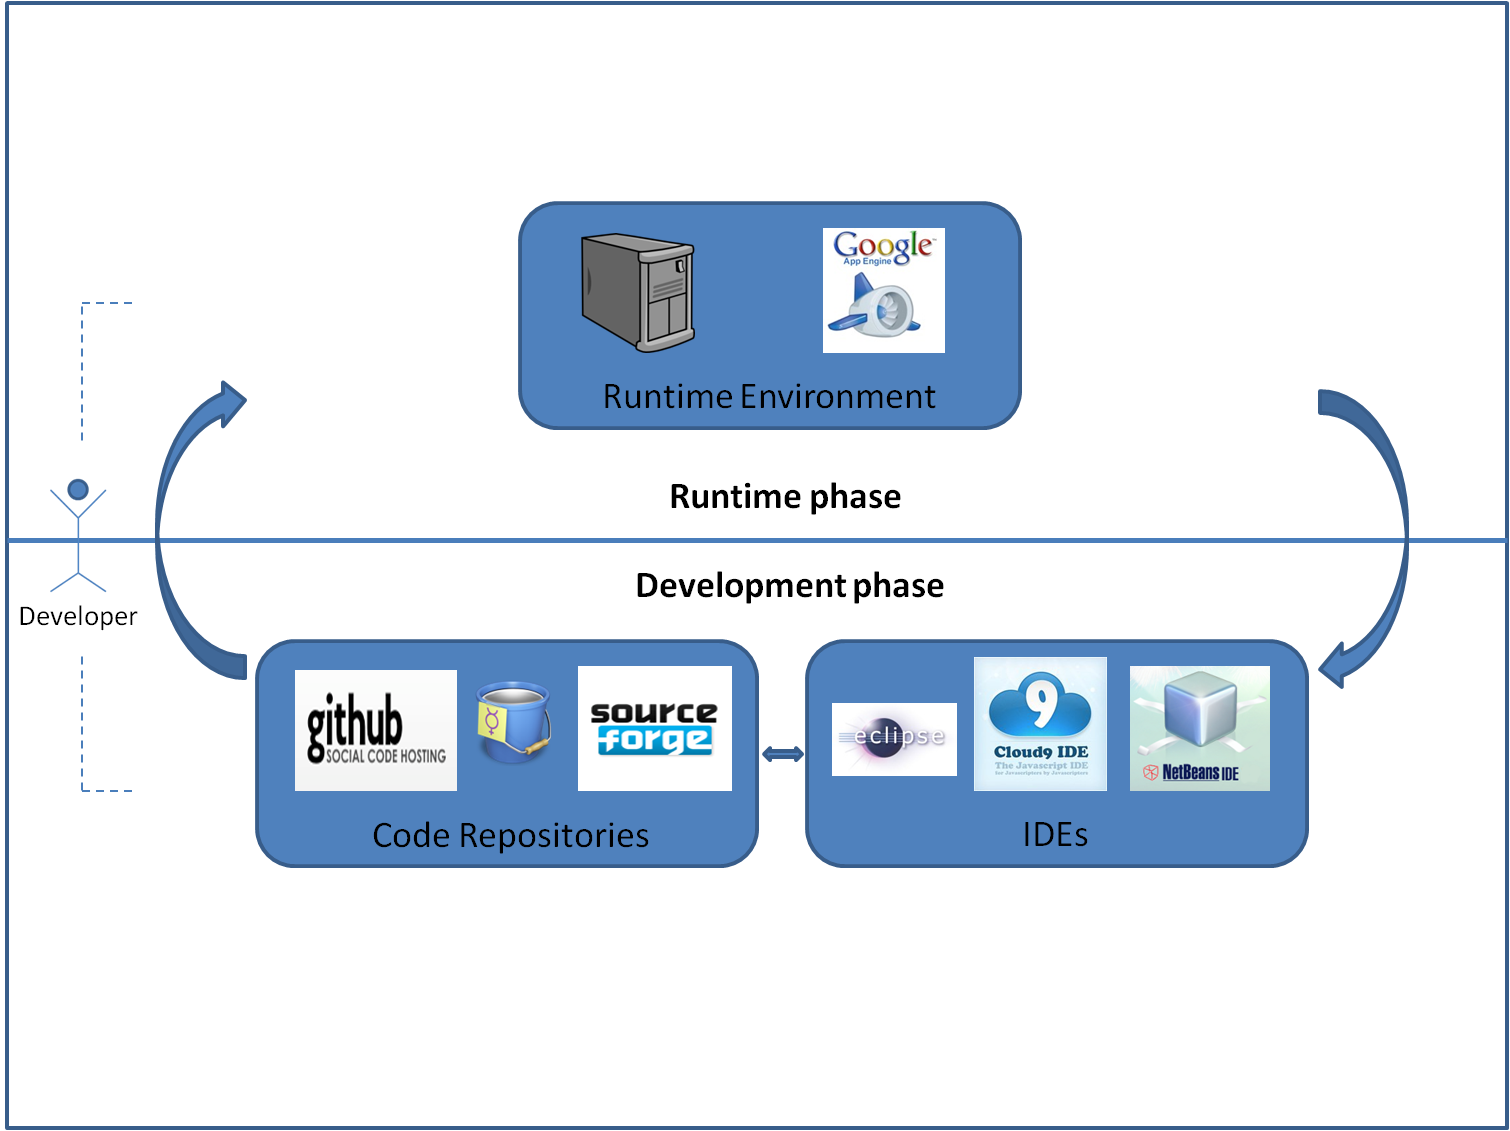
\includegraphics[width=0.7\columnwidth]{fig/Dev_Deploy}
\end{center}
\vspace*{-4ex}
\caption{Continuous Integration and Deployment of Software Applications.}
\label{fig:dev_deploy}
\end{figure}

% Software developers use project management tools, development frameworks, databases, etc., in their day-to-day software development tasks that help overcoming most obstacles, upfront. Some of these tools are primarily desktop-based (for example, the Eclipse IDE) while others are mostly Web-based (like Github). Making all these tools work together can be a pain, because each tool serves a specific purpose and there is a lack of interoperability among the tools, especially concerning data import and export.

% Developers spend good amount of time to optimize the entire development tools stack. Making all these tools work together perfectly can be a pain because each tool serves its own purpose and there is a lack of interoperability among the tools. Hence, developers spend good amount of time to optimize the entire software development stack.
%
% \begin{figure}[h]
% \begin{center}
% \includegraphics[width=0.6\columnwidth]{fig/softTools}
% \end{center}
% \vspace*{-4ex}
% \caption{Software Tools}
% \label{fig:softTools}
% \end{figure}

% Managing activities within a project using a variety of software tools make the software development process over the last years look quite different than it used to be. Developers are geographically distributed, they are agile and like to collaborate on different projects with other developers across the world. Code forges are a good example of global software development. It has gained a lot of attraction from the public and the software engineering community over the past decade. The success of these forges is highly dependent on the infrastructure provided to the developers and users in order to collaborate with each other~\cite{Shibuya:09} which helps increasing transparency, feedback, trust and tracking of dispersed software developers. They provide support for many software tools such as discussion forums, mailing lists, bug tracking systems, versioning systems, etc. Providing collaborative tools support in code forges promotes distributed software development. Imagine a group of developers would like to start a new project, they are not required to setup the necessary Web-based software tools internally because hosting or creating a project on a code forge automatically enables most of these software tools to the developers in order to collaborate with each other on the project.

Besides hosting of the project's source code and its related artifacts on the Web, the typical developer still carries out the actual development on her own machine using desktop-based environments. Imagine a developer who would like to work on multiple projects using different programming and database environments. She is required to configure the necessary desktop-based software tools such as an IDE before starting to contribute to a particular project. A developer who joins the team is also required to install and configure all the necessary software tools before being a productive member to the project. Last but not least, the transition to a new developer machine requires again installation and configuration of IDEs or development frameworks, which can turn out to be time-consuming. With the emergence of cloud infrastructure services, we have seen tremendous growth in adopting cloud services by leading IT organizations as their development and deployment infrastructure. The services offered by different providers covers almost all of the software tools which are required by the developers to carry out software development tasks. 
% We sketched the difference between the cloud-based and traditional desktop-based tools in the context of control and interoperability as shown in Fig.~\ref{fig:proximity_integration}.

\begin{figure}[ht!]
\begin{center}
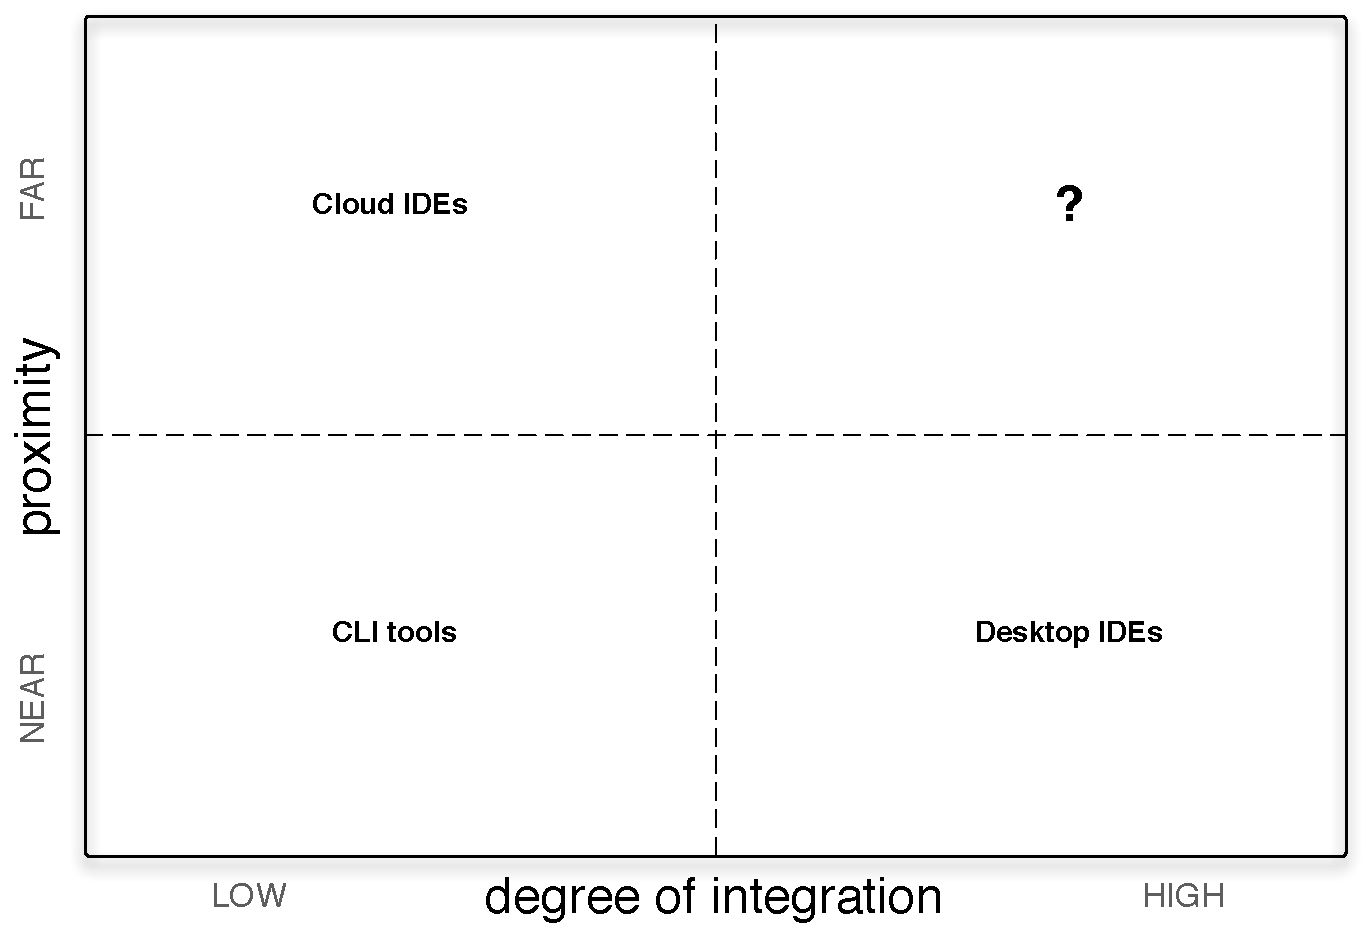
\includegraphics[width=0.6\columnwidth]{fig/proximity-vs-integration}
\end{center}
\vspace*{-4ex}
\caption{Categorization of software development tools.}
\label{fig:proximity_integration}
\end{figure}

In Fig.~\ref{fig:proximity_integration} we provide a categorization of software development tools along two dimensions:
\begin{enumerate}
	\item \textbf{Proximity}---indicates how much administrative control one has over the software tools: ``near'' means that the software tools are available locally (e.g., command-line tools, vi editor etc.), while ``far'' means the software tools are accessible via browser-based interface.
	\item \textbf{Degree of integration}---indicates how well the various software tools are integrated with each other: ``low'' means that there is little or no integration among software tools, while ``high'' means that the software tools are well-integrated with each other and support automation of tasks. For example, the Eclipse IDE supports integration with deployment tools such as Apache Tomcat~\cite{tomcat_url}) and build tools (e.g., Apache Ant~\cite{ant_url}).
\end{enumerate}

In this report, we first review and compare existing cloud-based development tools and IDEs in Section~\ref{sec:cbsd}. Then, in Section~\ref{sec:challenge}, we outline a roadmap of cloud-based software development by identifying  challenges and opportunities and propose a set of requirements for the next generation of cloud-based development tools. Finally, we conclude our work in Section~\ref{sec:conclusion}.


\section{Cloud-based Software Development Stack} \label{sec:cbsd}

With the emergence of cloud computing infrastructure, small and large corporations alike have started to move towards hosting their data, software applications, operational communication networks etc., on the large-scale server farms. Time and cost benefits are the leading motivating factors and measures for any business accessing tools and services via the cloud~\cite{Willie:11}.

Popular cloud computing services fit into one of the following categories: \emph{Infrastructure, Platform} or \emph{Software}. Software as a Service (SaaS)\footnote{\url{http://en.wikipedia.org/wiki/Software_as_a_service}} are offered by many service providers, including online project management applications, customer relation management, online office applications and many more. Following the successful adoption of cloud services by the enterprises, different cloud service providers started to offer data access, software, hardware and data storage services. Among them, few efforts takes ``as a service'' to the software development field where we get \textit{Development as a service (DaaS)}. DaaS is a suite of tools that allows to use traditional development practices for creating on-demand applications. DaaS expands the cloud computing development process to encompass external tools such as integrated development environments, source control systems and collaborative tools to facilitate development and deployment\footnote{\url{http://wiki.developerforce.com/page/An_Introduction_to_Metadata_and_Development_as_a_Service}} with the aim to facilitate and manage software tools and infrastructure for an enterprise, especially with development teams geographically distributed. By leveraging a cloud platform, an enterprise can start using software tools instantly, cost effectively and without managing any development infrastructure~\cite{Willie:11}. According to~\cite{Armbrust:CACM2010}, an enterprise can utilize cloud development infrastructure to:
\begin{enumerate}
        \item Scale on demand.
        \item Spend more resources on time-to-market by relieving resources from infrastructure management responsibilities.
        \item Achieve higher cost efficiencies.
        \item Configure development infrastructure in minutes rather than spending whole day on an installed infrastructure.
\end{enumerate}

Recently, service providers have started to offer browser-based development environment, allowing to edit, test, debug, deploy and manage applications using the browser without the need of installing or configuring any tool on a local machine. It enables developers to harness the cloud computing power: just as Platform-as-a-Service\footnote{\url{http://en.wikipedia.org/wiki/Platform_as_a_service}} (PaaS) enables an enterprise to run applications in the hosted platforms, DaaS provides a new software development stack\footnote{Kudos to Mike Amundsen for coining the term ``cloud-stack'' programming in his blog post available via: \url{http://www.amundsen.com/blog/archives/1116}} giving developers the power to write, deploy and manage software applications in the cloud as depicted in Fig.~\ref{fig:DevStack}:

\begin{figure}[h]
\begin{center}
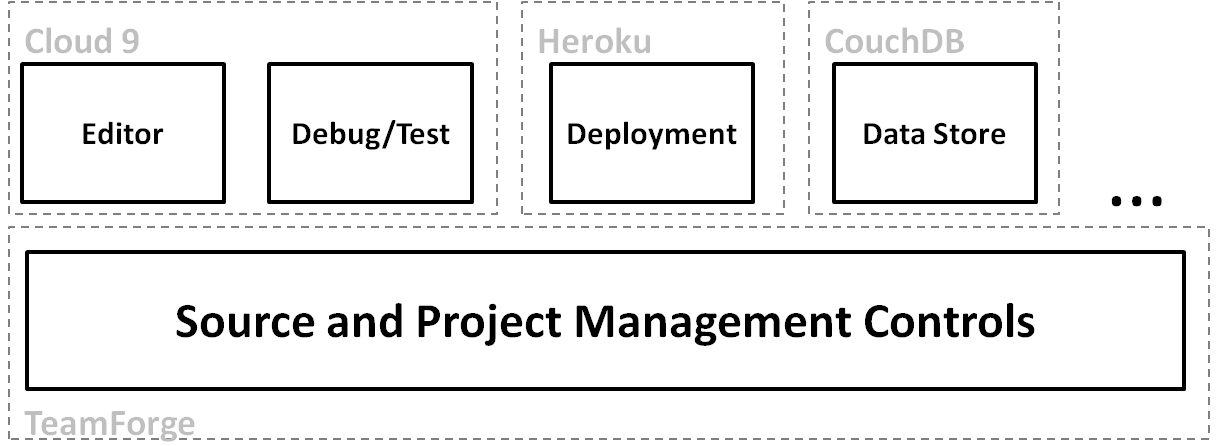
\includegraphics[width=0.8\columnwidth]{fig/CloudDevStack}
\end{center}
\vspace*{-4ex}
\caption{Cloud-based Software Development Stack.}
\label{fig:DevStack}
\end{figure}

The cloud-based software development stack typically comprises the following components (exemplary coverage overlaid in  Fig.~\ref{fig:DevStack}):

\begin{enumerate}
    \item \textbf{Editor}---A browser-based code editor, allowing to edit, debug and test source code, for example, Cloud9 IDE~\cite{cloud9IDE_url}.
    \item \textbf{Deployment}---Deployment of an end-user application in the cloud through a PaaS provider, such as Heroku~\cite{Heroku_url}.
    \item \textbf{Data Store}---A cloud-based data storage system (RDBMS or NoSQL) used by an application to store and query application data, for example CouchDB~\cite{couchdb_url}.
    \item \textbf{Source and Project Management Controls}---Managing and sharing software repositories through cloud-based collaborative software development architecture, such as TeamForge~\cite{teamforge_url}.
\end{enumerate}

In the following we will review each component of the cloud-based software development stack and outline their features and limitations.
%These browser-based IDEs allows developers to write code, save, build and run the applications in the cloud.

\subsection{Browser-based IDE} \label{sec:ides}

From the software development perspective, the ability to write, build and deploy a software application using only a browser is a promising approach. This shift of writing code directly in browser-based IDEs is getting more and more attention recently with some trailblazing examples such as Ace~\cite{ace_url}, Cloud9, Orion~\cite{orion_url}, SourceKit~\cite{sourcekit_url}, BrainEngine~\cite{brainengine_url} and CodeMirror~\cite{codemirror_url} making impressive advancements\footnote{\url{http://blogs.developerforce.com/developer-relations/2011/03/browser-based-ides.html}}. Service providers offer single component or a combination of components as shown in the cloud-based software development stack (Fig.~\ref{fig:DevStack}). In the beginning, browser-based IDEs were considered nothing more than a text editor with syntax highlighting but these online IDEs are more than that, nowadays: they offer a hosted development environment where developers can develop their Web applications in JavaScript, Java, PHP, Python, Ruby, etc. The platform runs in the browser and lives in the cloud, allowing development teams run, debug and deploy applications from anywhere, anytime. It enables developers to easily start projects behind a single URL, share their code, and collaborate with co-developers all over the world without having to install anything on the client. It also supports syntax highlighting for most popular languages as well as parses and analyze the code in the background and points out any errors in the code if exists. Besides allowing developers to write programs in different programming languages, browser-based IDEs also supports agile and collaborative software development processes. It facilitates collaboration by allowing developers to chat and collaborate with other fellow developers without leaving the browser-based IDE (see Fig.~\ref{fig:Cloud9}). Few browser-based IDEs also supports integration with code forges (e.g., GitHub) to support versioning, maintenance and sharing source code online.

\begin{comment}
\textbf{Cloud9 enables developers to easily start projects behind a single URL, share their code, and collaborate with co-developers all over the world without having to install anything on the client. The platform runs in the browser and lives in the cloud, allowing development teams run, debug and deploy applications from anywhere, anytime. The DaaS also offers syntax support for popular programming languages; the ability to simultaneously collaborate on code and projects; the ability to run, realtime code analysis; the ability to debug and test applications; and includes GitHub, Bitbucket and Joyent integration\footnote{\url{http://techcrunch.com/2011/06/21/development-as-a-service-platform-cloud9-raises-5-5m-from-accel-and-atlassian-software/}}. It brings the interesting concept of (Software) Development As A Service, so that the software development Components can be provisioned as a service, using the Cloud-based model\footnote{\url{http://cloudcomputing.sys-con.com/node/1703703}}}
\end{comment}

\begin{figure}[h]
\begin{center}
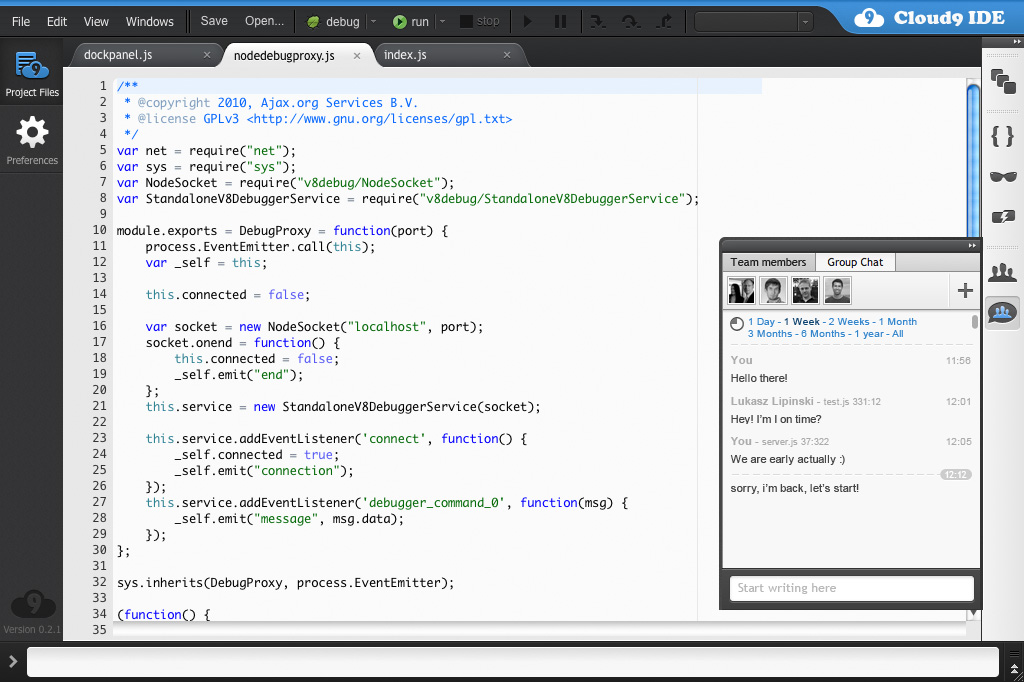
\includegraphics[width=0.8\columnwidth]{fig/Cloud9}
\end{center}
\vspace*{-4ex}
\caption{Cloud9 IDE taken from~\cite{cloud9IDE_url}.}
\label{fig:Cloud9}
\end{figure}

\subsubsection{Comparison of browser-based IDEs}

In the following we compare browser-based IDEs as example of cloud-based software development components. The browser-based IDEs are selected without any preference and are listed in no particular order (cf. Table~\ref{DaaS_comparison}). We compare them in terms of programming language support, source control integration, project collaboration features as well as deployment options. Developing code directly in the cloud should enable developers to deploy the application into the cloud, we will see which browser-based IDEs supports application deployment. Quite often, a software project is developed by a team of developers who are geographically distributed; we will see which browser-based IDEs currently supports the social collaboration aspect.

\begin{table}[h]
\centering
\tiny {
\begin{tabular}{|p{2.3cm}|p{4.0cm}|p{2.5cm}|p{1.5cm}|p{1.5cm}|p{1.2cm}|}
\hline
\tiny \textbf{Product} & \tiny \textbf{Language} & \tiny \textbf{Source Control Integration} & \tiny \textbf{Project Collaboration} & \tiny \textbf{Deployment}\\
\hline
CodeRun~\cite{codeRun_url} & C\#/PHP/JavaScript/HTML & No & Yes & Yes \\
\hline
Cloud9 & Ruby/PHP/JavaScript/HTML & Yes & Yes & Yes \\
\hline
eXo Cloud & Java/PHP/Ruby/JavaScript/HTML & Yes & Yes & Yes \\
\hline
Bespin~\cite{bespin_url} & JavaScript/HTML/CSS & No & Yes & No \\
\hline
Kodingen~\cite{kodingen_url} & PHP/Perl/Python & Yes & Yes & No \\
\hline
Bungee Connect~\cite{bungee_url} & custom written language & Yes & No & Yes \\
\hline
codeanywhere~\cite{codeanywhere_url} & PHP/CSS/JavaScript/HTML & No & No & No \\
\hline
ECCO~\cite{ecco_url} & PHP/Java/JavaScript/HTML & No & No & No \\
\hline
WonderFL~\cite{wonderfl_url} & Action Script3 & No & Yes & No \\
\hline
\end{tabular}
}
\caption{Comparison between browser-based IDE(s).}
\label{DaaS_comparison}
\end{table}

As shown in Table~\ref{DaaS_comparison}, all browser-based IDEs support Web standard scripting languages although few of them also support object oriented languages such as Java. Version tracking on source code is an important asset in software development but not all browser-based IDEs currently support it. Regarding social collaboration aspect, few browser-based IDEs support project collaboration allowing developer to share his/her workspace with other fellow developers in order to collaborate with each other.

Comparing the current state of features offered by browser-based IDEs with Fig.~\ref{fig:dev_deploy}, we can conclude that browser-based IDEs still require improvements in their design and features. Only few browser-based IDEs support integration with code repositories. Moreover, they do not support all programming-languages. For example, IDEs like \texttt{Cloud9}, \texttt{eXo Cloud} etc., fit best into the continuous development and deployment architecture (cf. Fig.~\ref{fig:dev_deploy}) but it does not suit Python developers due to no support for Python programming-language. Contrary to that, \texttt{Kodingen} does support Python programming-language but does not support integration with code repositories and deployment of applications in the cloud. Hence, Python developers are unable to get the best from using browser-based IDEs under consideration.

With browser-based IDEs, developing and deploying applications become much more streamlined and enables cloud platforms easily accessible to the developers. These Web-based programming environments can (nearly) replace our desktop IDEs and code editors. They support most of the programming languages available to date as well as allows developers to start connecting to each other into the cloud and build up teams in a way that they couldn't be able to do before, hence giving them more freedom to organize their team development. Apart from team building and programming language support, it offers convenience, pace -- the ability to ramp up a project in the order of minutes rather than days or weeks which is a huge benefit. Contrary to the benefits which browser-based IDEs has brought into software development field, there is still room for improvement in these IDEs before it is widely adopted. In this section, we only highlighted some limitations of browser-based IDEs and further compared their features against each other as shown in Table~\ref{DaaS_comparison}.
%Although we have listed down features, limitations and compare few browser-based IDEs (cf. Table~\ref{DaaS_comparison}), there are also many PaaS providers available to date which offers variety of software services to run or deploy software applications.


\subsection{Deployment in the Cloud}

Cloud-based infrastructure has changed the way applications were built and deployed. Platform-as-a-Service (PaaS) offer services with a primary focus on simplifying and accelerating the entire software application development lifecycle, making it easier and robust than ever to build, run and deploy applications. It provides a browser-based interface to allow application providers to select the software stack, relational databases, application frameworks etc., without installing or configuring anything as shown in Fig.~\ref{fig:Jelastic}. Using PaaS, application deployment is only a matter of uploading the application package (e.g. *.war file) to the selected environment with no extra coding or configurations required. PaaS providers also provides versioning on deployments so that the application provider can deploy an older version of the application, if necessary. In short, building and deploying applications in the cloud brings a  non-exhaustive list of benefits as follows:

\begin{enumerate}
	\item Scalability
	\item Faster development and deployment
	\item Reliability
	\item Managing applications via single console
\end{enumerate}	

\begin{figure}[h]
\begin{center}
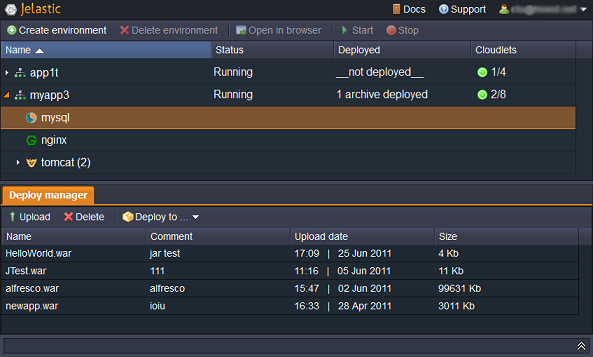
\includegraphics[width=0.8\columnwidth]{fig/Jelastic}
\end{center}
\vspace*{-4ex}
\caption{Jelastic Environment Manager taken from~\cite{jelastic_manager_url}.}
\label{fig:Jelastic}
\end{figure}

\subsubsection{Comparison of PaaS providers}

In the following we take into consideration few PaaS providers as example of cloud-based software development components (Table~\ref{PaaS_comparison}): we compare them in terms of programming-language support, continuous integration tools as well as data storage services because we believe that these tools/frameworks are important assets of software development. Build integration is an important tool for building large and complex software systems which is the reason we selected this particular feature for comparing different PaaS providers. Most applications deal with some sort of storage medium to store and later query data from it. We list down which storage formats are supported by different PaaS providers under consideration. The PaaS providers in Table~\ref{PaaS_comparison} are selected without any preference and are listed in no particular order.
%In Table~\ref{PaaS_comparison}, we listed down few PaaS providers and the programming languages they support for deployment. It provides a glimpse of what PaaS provider could be a best fit for software development organizations who are thinking about adopting cloud deployment infrastructure.

\begin{table}[h]
\centering
\tiny {
\begin{tabular}{|p{2.3cm}|p{4.5cm}|p{2.5cm}|p{2.5cm}|p{1cm}|}
\hline
\tiny \textbf{Product} & \tiny \textbf{Language} & \tiny \textbf{Build/Continuous Integration} & \tiny \textbf{Data Storage}\\
\hline
CloudBees~\cite{CloudBees_url} & Java/Spring/JRuby/Grails/Groovy/Scala & Yes & SQL/NoSQL \\
\hline
OpenShift~\cite{OpenShift_url} & PHP/Python/Ruby/Perl/Node.js/JBoss & Yes & SQL/NoSQL \\
\hline
Heroku~\cite{Heroku_url} & Ruby/Node.js/Closure/Java/Python/Scala & Yes & SQL/NoSQL \\
\hline
Jelastic~\cite{jelastic_url} & Java/JRuby/Groovy/Scala/ColdFusion & No & SQL/NoSQL \\
\hline
Google App Engine~\cite{googleapp_url} & Java/Python/JRuby/Scala/Django & No & SQL/Proprietary \\
\hline
dotCloud~\cite{dotcloud_url} & PHP/Python/Java/Perl/Node.js/Ruby & No & SQL/NoSQL \\
\hline
Azure~\cite{azure_url} & .Net/Node.js/Java/PHP & No & SQL/NoSQL \\
\hline
CloudFoundary~\cite{CloudFoundry_url} & Spring/Ruby/Grails/Node.js/Scala & No & SQL/NoSQL/Key-Value \\
\hline
\end{tabular}
}
\caption{Comparison between PaaS providers.}
\label{PaaS_comparison}
\end{table}

As depicted in Table~\ref{PaaS_comparison}, most PaaS providers offers support for many different programming and scripting languages while few of them only supports JVM-based languages (e.g., CloudBees, Jelastic). Many PaaS providers under consideration is not supporting build integration services currently which we believe is the downside of these PaaS providers. The reason is we are focusing on a desktop-less software development environment where we consider browser-based IDEs as our code editor for writing applications. Hence, we believe that build integration tools and frameworks must be provided by the PaaS providers. Most PaaS providers under consideration supports both SQL and NoSQL storage format with the exception of \texttt{Google App Engine} which also provides its own proprietary storage format (i.e., Big Table). By comparing the set of features currently offered by PaaS providers with Fig.~\ref{fig:dev_deploy}, we can conclude that the services offered by PaaS providers are pretty much aligned with the needs of enterprises and also make them free from the hassle of managing infrastructure requirements.

\subsection{Cloud-based Project Management Tools}

With the growing interest in the usage of cloud-based infrastructure services, many service providers have started to offer cloud-based developer-related services specially for enterprises having distributed teams across the globe, hence freeing them from the hassle of deploying and hosting project management tools and frameworks internally. Developer-related services essentially covers the Application Lifecycle Management\footnote{\url{http://en.wikipedia.org/wiki/Application_lifecycle_management}} (ALM) which radically simplifies management of software projects. Using cloud-based infrastructure, provisioning of project management tools can be done in minutes and scale easily without having to invest time and energy on managing the infrastructure. 

\subsubsection{Comparison of Cloud-based Project Management Tools}
In the following we take into account few project management tool providers as example of cloud-based software development components (Table~\ref{prjtools}): we compare them in terms of support for different project management tools which developers interact with in their day to day software development tasks. The service providers are selected without any preference and are listed in no particular order.

\begin{table}[h]
\centering
\tiny {
\begin{tabular}{|p{2cm}|p{2cm}|p{2.5cm}|p{2.5cm}|p{2.5cm}|}
\hline
\tiny \textbf{Product} & \tiny \textbf{Version Control} & \tiny \textbf{Build/Continuous Integration} & \tiny \textbf{Social Collaboration} & \tiny \textbf{Project Planning/Tracking}\\
\hline
TeamForge & Yes & Yes & Yes & Yes \\
\hline
OnDemand~\cite{atlassian_url} & Yes & Yes & Yes & Yes \\
\hline
JazzHub~\cite{jazz_url} & Yes & No & Yes & Yes \\
\hline
AccuRev~\cite{accurev_url} & Yes & Yes & Yes & Yes \\
\hline
\end{tabular}
}
\caption{Comparison between cloud-based project management tools.}
\label{prjtools}
\end{table}

As shown in Table~\ref{prjtools}, service providers under consideration covers all major project management tools with the exception of JazzHub which does not support build integration. Although it is customized specifically for academic research and classroom projects which might be the reason for exclusion of certain features comparing to other service providers. Comparing the features of these cloud-based development tools with Fig.~\ref{fig:dev_deploy}, we can conclude that it pretty much covers everything required for continuous integration and development infrastructure. Though, cloud-based project management services are designed primarily to offer services to enterprises (which mostly works on closed-source projects), that could be the reason we don't see integration of such project management services with code repositories such as GitHub.

In the next section, we will discuss challenges concerning cloud-based tools and IDEs along with potential features which they could take into consideration to gain a competitive advantage.


\section{Towards a Future Generation of Cloud Development} \label{sec:challenge}

%\section{Challenges and Opportunities} \label{sec:challenge}

In traditional in-house software development, we deal with different software repositories which surround a particular project. These software repositories are necessary to maintain and execute a project in an structured way. As we have discussed the emerging trends of cloud-based infrastructures to support software development (cf. section~\ref{sec:cbsd}) and the different browser-based development tools/frameworks and IDEs which are available to date (cf. Table~\ref{DaaS_comparison}, Table~\ref{PaaS_comparison}, Table~\ref{prjtools}), we foresee the development of software projects in the cloud as depicted in Fig.~\ref{fig:cloudDevDeploy}. 
%These plugins pulls project related information from different software repositories and present it in the developer's favorite desktop IDE instead of forcing him/her to leave the desktop IDE.

\begin{figure}[h]
\begin{center}
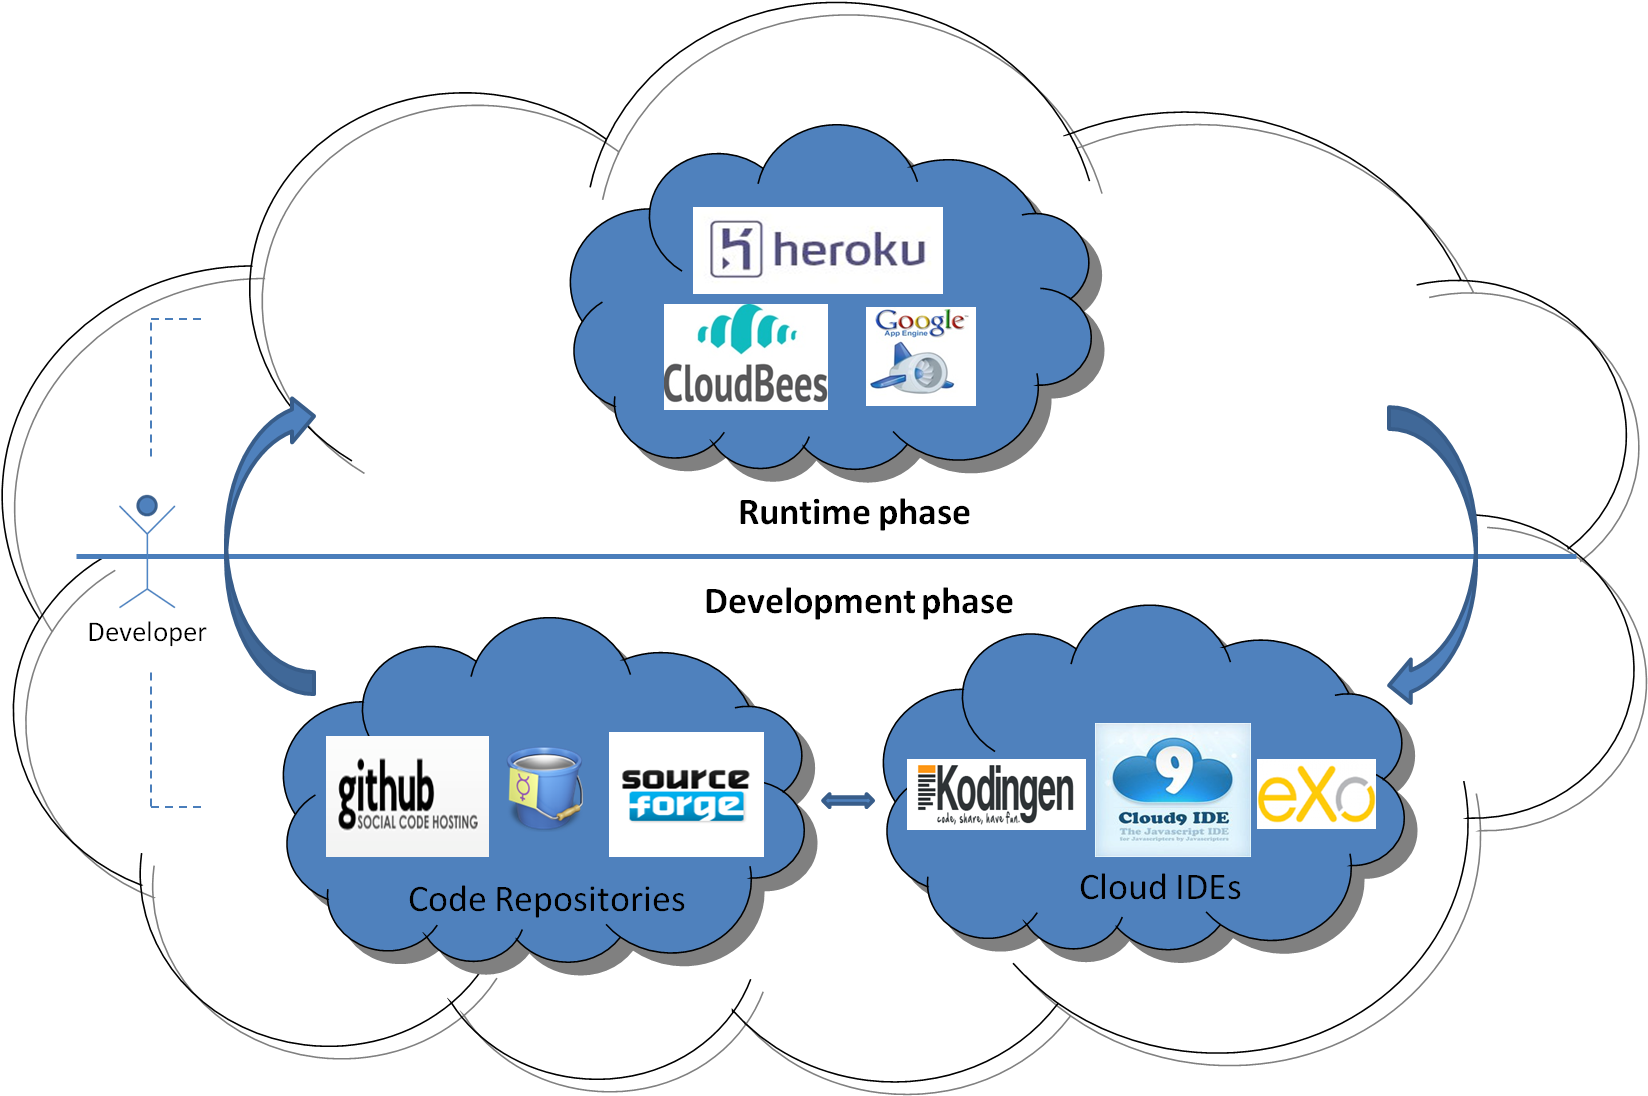
\includegraphics[width=0.8\columnwidth]{fig/cloud_Dev_Deploy}
\end{center}
\vspace*{-4ex}
\caption{Continuous Integration and Deployment of Software Applications in the Cloud.}
\label{fig:cloudDevDeploy}
\end{figure}

\subsection{Challenges and Opportunities}
These browser-based IDEs do have limitations: most focus on Web application development using only HTML, JavaScript etc., others support Web application development using Java etc. Further, support for accessing other software repositories is lacking, which is quite often necessary to manage large projects. In the following we discuss challenges or areas of improvement which can foster the adaption of browser-based software development:

\begin{enumerate}
    \item \textbf{Dealing with the agile software development life-cycle.} In agile software development, immediate feedback is essential and it is generated through frequent commits, builds, testing and continuous integration. As the cloud-based development infrastructure offers support for these software tools as a single integrated platform (cf. Table~\ref{prjtools}), it is worth investigating if the online browser-based IDE adds more efficiency, support and transparency than developing the code in a desktop-based environment. Currently, cloud-based software development tools offer integration with desktop-based development environments but such type of integration is missing with browser-based IDEs. In order to fully support agile software development in the cloud we need to support integration between different cloud-based development tools and infrastructures.
    \item \textbf{Automation of tasks.} Cloud-based infrastructure makes it straight-forward to export and share data from software tools (i.e., coding, testing, build logs, integration tests etc.). Real time capturing of data from these tools will enable enterprises as well as developers to measure performance, tracking activities of a developer and monitoring the overall progress on the project. In order to achieve this, service providers must provide plugins/tools which can publish and consume data from different cloud-based development tools.
    \item \textbf{Integration with code forges.} Hundreds of thousands of projects are hosted on different code forges. Only few browser-based IDEs do support integration with code forges (e.g., Cloud9 supports GitHub integration). Integration with code forges will enable developers to easily work on software projects which are already hosted on these code forges, using browser-based IDE. As code forges hosts a variety of project management tools (i.e., bug tracking systems, mailing lists, discussion forums), it will further assist developers to reuse the existing project management tools hosted on these code forges. For example, a bug could be fixed by modifying the source code in a browser-based IDE, compiling, building, testing and later pushing the changes back to the code forge along with changing the status of a bug on the code forge.
        %Additionally, if the cloud services are down due to some reasons than the development tasks can still be carried out by downloading from code forge and working on the code locally.
    \item \textbf{Bridging the ``off-line gap''.} Browser-based IDEs should allow developers to import or export projects directly from their desktop IDEs to the cloud. A developer should be able to code on his local machine and a single push button would allow him to push the changes to the cloud so that other team members can access or review the code changes using browser-based IDE. In the same direction the question has to be answered how (local or remote) backup are supported.
\end{enumerate}

\subsection{Requirements} \label{sec:requirements}
Based on the previous section we have derived a set of requirements we consider pivotal for the next generation of cloud-based software development tools.
\begin{enumerate}
	\item The integration between PaaS and cloud-based development tools is essential; the interfaces should be standardised, both on the data format level (for example, JSON) as well as on the protocol level (RESTful).
	\item Cloud-based development tools (such as build integration, project planning etc.) must support integration with browser-based IDEs.
	\item Browser-based IDEs should support interfaces allowing real-time capturing of a developer's activity in a project to promote awareness among co-developers.
	\item Browser-based IDEs must provide interfaces to enable integration with code forges to support open source software development in the cloud.
	\item Integration between desktop-based and browser-based IDEs should be supported. This can include import and export of projects as well as configuration settings.
\end{enumerate}


\section{Conclusion} \label{sec:conclusion}
In this report, we have established a cloud-based development stack and reviewed browser-based IDEs that can bring a significant change in the way software development is carried out. With the existing browser-based IDEs, \emph{small applications } can be easily written and deploy, however we believe that they are not ready yet for prime time to handle large software projects. We have identified a number of challenges in the cloud-based development stack, especially concerning the browser-based IDEs, which might hamper their take-up and proposed a roadmap towards a new generation of cloud-based software development tools.


\bibliographystyle{alpha}
\bibliography{tr_cloud-SD}

% \clearpage
%
% \appendix
%
% \section{Appendix: Tools and Applications}
% \label{app:toolsnapps}

\begin{comment}
Some pointers on developing in the cloud:
http://alan.blog-city.com/developing_in_the_cloud_without_falling.htm
http://www.infoworld.com/d/cloud-computing/developing-cloud-apps-whats-different-675
http://cloudcomputing.sys-con.com/node/1870656
http://www.aservo.com/fileadmin/user_upload/ag/downloads/downloadcenter/developer/SoftwareDevelopmentInTheCloud.pdf
\end{comment}
\end{document}
